\section{Milky Way halo}\label{sec:theory:MWALP}

\subsection{Virialized dark matter halo}

In the SHM\,\cite{Evans2019_SHMRefined}, the Milky Way dark matter population is treated as a virialized\footnote{The term ``virialized'' means that the dark matter is gravitationally bound. } ensemble. 
In the Galactic rest frame, the dark-matter velocity distribution is approximated by a Maxwell--Boltzmann distribution truncated near the Galactic escape speed\,\cite{Evans2019_SHMRefined}.
The average speed of local dark matter\footnote{Here, ``local'' refers to the solar radius in the Milky Way.} is $v_\mathrm{DM} \approx \SI{220}{\km\per\s}$.
The local dark matter density is estimated to be $\rho_{DM}\approx\SI{0.4}{\GeV\per\centi\meter^3}$. 
The Rabi frequency $\Omega_a$ can be computed from Equations\,\eqref{eq:a0_rhoDM}, \eqref{eq:ALP_field}, and \eqref{eq:HaNN}:
\begin{equation}
    \Omega_a
    = \dfrac{1}{2\hbar} g_{\mathrm{aNN}} a_0 m_a c v_{\bot}
    \approx \dfrac{1}{2} g_{\mathrm{aNN}}
    \sqrt{2\hbar c \rho_{DM}}\,v_{\bot}
    \,.
    \label{eq:Omega_a_MW}
\end{equation}
Here it is assumed that the ALP-field gradient comes exclusively from the relative motion of the field and the detector. 
It is important to note that the ALP field is a stochastically varying quantity\,\cite{Centers2021Stochastic}, so that the $\Omega_a$ in Equation~\eqref{eq:Omega_a} is the root-mean-squared (rms) value.
For $v_{\bot} = \SI{220}{\km\per\second}$, $\Omega_a/2\pi=g_{\mathrm{aNN}}\times\SI{0.2}{\GeV\cdot\Hz}$.
For an experiment searching for $g_{\mathrm{aNN}}\leq 10^{-10}\,\SI{}{\per\GeV}$, the Rabi period is $2\pi/\Omega_a \geq 1000\,\mathrm{yr}$; the ALP-field gradient is therefore a weak drive on the spins.

Though it is named ``standard'' halo model, it is not a complete description of the Milky Way dark matter halo, but focuses on the dark matter properties at solar radius. 
It is more of a model built on phenomenological observations, rather than a model tested through direct measurements. 
Not every question about the Milky Way halo can be answered by the SHM. 
For example, the SHM does not account for the presence of substructure in galaxies. 
There have been alternative models or modifications to the SHM, including SHM$^{++}$\,\cite{Evans2019_SHMRefined}, caustic rings\,\cite{Sikivie1998_CausticRings}, and the presence of substructure in the form of streams\,\cite{Freese2004_Streams,Savage2006_Streams,Kuhlen2010_Streams,Lisanti2011_Streams}. 
In these models, the local dark matter density and velocity distribution can be significantly different from the SHM. 
These alternative models will be accounted for in the future work of the CASPEr. 

\subsection{Stochasticity due to inteference}\label{sec:theory:MWALP:stochasticity}

If the ALP constitutes the dominant component of the Milky Way dark matter, the local ALP field is a superposition of many modes with different velocities and phases. 
Here the phases of the occupied modes are assumed to be uncorrelated.
Each velocity class contributes one term to the multimode field in Equation~\eqref{eq:ALP_sum}, with
\begin{equation}
    \nu(\mathbf{v})
    =\frac{m_a c^2}{h} \left(1 + \frac{v^2}{2c^2}\right),
    \qquad
    \mathbf{k}(\mathbf{v})=\frac{m_a\mathbf{v}}{\hbar}
    \,.
\end{equation}
The relative spread of velocities is on the order of $v_a/c \sim 10^{-3}$.
Due to the second-order Doppler effect, the relative spread of kinetic energies is on the order of $(v_a/c)^2 \sim 10^{-6}$. 
The inverse of this spread is defined as the quality factor of the ALP field, $Q_a =(c/v_a)^2 \sim 10^6$.
Therefore, in the frequency domain, the ALP field is a narrowband signal with a fractional linewidth $\Delta\nu_a/\nu_a \sim 10^{-6}$. 
Considering the Maxwell--Boltzmann velocity distribution, the sum of the modes as shown in \eqref{eq:ALP_sum} is a random walk in the complex $\Psi$ plane: the two quadratures approach Gaussian random variables, while the field (average) envelope follows a Rayleigh distribution\,\cite{Centers2021Stochastic,Gramolin2022Feb_SpectralSignatures}. 
Consequently, in the time domain, the ALP field is a coherent oscillation only on times short compared with its coherence time; on longer time scales, the amplitude and phase drift stochastically, due to the spread of frequencies in the multimode superposition. 
The ALP coherence time $\tau_a$ can be estimated by the quality factor
\begin{equation}
    \tau_a = \frac{2\pi Q_a}{\nu_a}
    \,.
    \label{eq:taua_Qa_nua}
\end{equation}
% Within one coherence time, the superposition in Equation~\eqref{eq:ALP_sum} is well approximated by the coherent mode in Equation~\eqref{eq:ALP_field}.
% On longer time scales, the random phases between modes cause the amplitude and phase of the effective oscillation to drift, so the field must be treated as a stochastic process\,\cite{Centers2021Stochastic}.
% For Compton frequencies above \SI{1}{\kHz}, $\tau_a \lesssim \SI{1000}{\second}$; the interplay between $\tau_a$ and the NMR relaxation times determines the optimal measurement strategy in Chapter~\ref{chap:results}.
% The continuous velocity distribution therefore maps directly onto a continuous frequency distribution.
One example of stochasitc AlP field in time and frequency domains is shown in Figure~\ref{fig:MW_axion_time_domain_stochastic}. 


\begin{figure}
    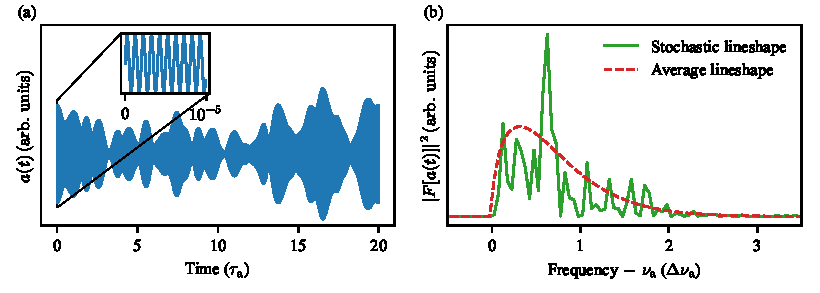
\includegraphics[width=0.99\textwidth]{figures/MW-axion-time-frequency-domain.pdf}
    \caption{
    Simulated axion fields in the time and frequency domains. 
    (a) Time-domain axion field $a(t)$, with a magnified view showing the oscillation at axion Compton frequency in the inset. 
    The envelope of the $a(t)$ changes over time, indicating the coherence time $\tau_a$ is finite. Here $\tau_a$ is chosen as $Q_a / \nu_a $. 
    (b) The stochastic lineshape in the frequency domain is computed as $|F[a(t)]|^2$, where $F[a(t)]$ denotes the Fourier transform of the time-domain signal shown in (a). 
    The average lineshape represents the expected amplitude spectrum after sufficient averaging. 
    The linewidth $\Delta \nu_a$ is approximated as $\nu_a / Q_a $.
    The figure is generated by the script \url{scripts-and-data/MW-axion-time-frequency-domain.py}. 
    Reproduced from Ref.\,\cite{YGK2026_CavityLumpedSpin} with permission. }
    \label{fig:MW_axion_time_domain_stochastic}
\end{figure}

\subsection{Periodic modulations}\label{sec:theory:MWALP:modulations}

% sensitive axis of CASPEr-G
In the resonance scheme, CASPEr-G is only sensitive to the component of $\boldsymbol{\nabla}a$ perpendicular to the bias field $\mathbf{B}_0$.\footnote{This is sometimes defined as the sensitive axis of a haloscope. However, sensitive axis is also defined as the axes perpendicular to the bias field. Due to the ambiguity in the definition, the term ``senstive axis'' is avoided in this thesis.}
The bias field is always veritcal with repect to the ground. 
Therefore, the ALP-gradient-driven spin precession depends on the direction of the relative velocity between the Earth and the local dark-matter halo.
The Earth's rotation and orbital motion modulate this relative velocity, and give rise to daily and annual modulations of the ALP signal, respectively.

% Daily and annual modulation
As the Earth rotates, this direction sweeps through space with a period of one sidereal day.
An ALP signal therefore exhibits a daily modulation of its amplitude and phase\,\cite{Gramolin2022Feb_SpectralSignatures}.
In addition to daily rotation, the Earth's orbital velocity around the Sun modulates the relative ALP-detector velocity with a period of one year.
Both the daily and annual modulations have precisely predictable periods and phases, making them useful consistency checks for any claimed dark-matter-candidate signal.
Examples of daily and annual modulations are shown in Figure~\ref{fig:MWAxion-annual-daily-modulations}. 

\begin{figure}
    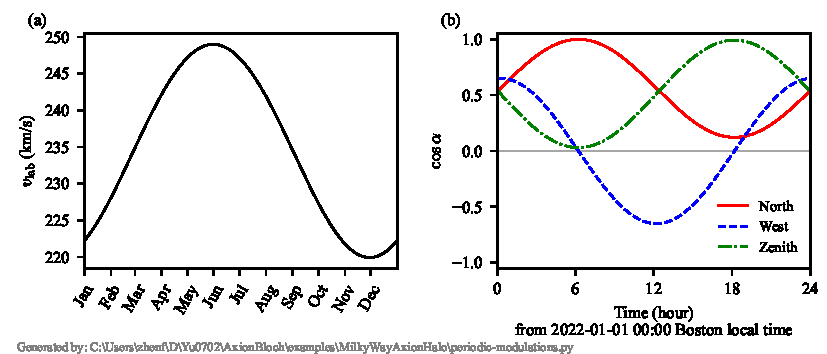
\includegraphics[width=0.99\textwidth]{figures/MWAxion-annual-daily-modulations.pdf}
    \caption{Periodic (annual and daily) modulations. (a) Annual modulation of laboratory speed due to the Earth's orbital motion around the Sun. (b) Daily modulations of angles between the ALP field and the three orthogonal orientations: towards the north, the west, and the zenith. The location is the Boston University and the date is January 1 (local time). \YZ{can we use figure width 6 or 6.5 for making font larger? TODO}. The plot is reproduced from Ref.\,\cite{Gramolin2022Feb_SpectralSignatures} with permission.}
    \label{fig:MWAxion-annual-daily-modulations}
\end{figure}


% \subsection{Numerical simulation}\label{sec:theory:MW:simulation}

% \YZ{include several important examples and give a summary of signal dependence. }
